\documentclass[border=3pt,tikz]{standalone}
\usetikzlibrary{arrows}
\usetikzlibrary{positioning}
\usetikzlibrary{calc}
\usetikzlibrary{arrows}
\usetikzlibrary{decorations.pathreplacing}
\begin{document}
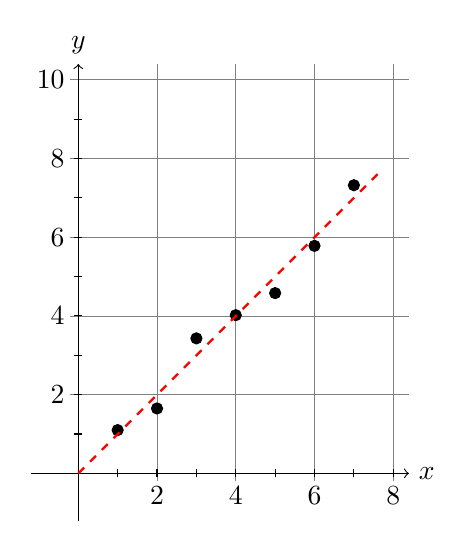
\begin{tikzpicture}
    \draw[very thin,color=gray] (-0.1,-0.1) grid (4.2,5.2);
    
    \draw[->] (-0.6, 0) -- (4.2,0) node[right] {$x$};
    \draw[->] (0,-0.6) -- (0,5.2) node[above] {$y$};
    
    \foreach \x in {1,...,8}
    {
      \draw[thin] (\x / 2, 0.05) -- (\x /2, -0.05);
      }
    
    \foreach \x in {2, 4, 6, 8}
    {
      \node[below]  at (\x /2 , -0.05) {$\x$};
      }
    
    \foreach \y in {1,...,9}
    {
      \draw[thin] (0.05 , \y / 2) -- (-0.05 , \y /2);
      }
    
    \foreach \y in {2, 4, 6, 8, 10}
    {
      \node[left]  at (-0.05, \y / 2) {$\y$};
      }
    
    \filldraw[black] (0.5,1.1 /2) circle (2pt);
    \filldraw[black] (2/2, 1.65 /2) circle (2pt);
    \filldraw[black] (3/2, 3.43/2) circle (2pt);
    \filldraw[black] (4/2, 4.02/2) circle (2pt);
    \filldraw[black] (5/2, 4.58/2) circle (2pt);
    \filldraw[black] (6/2, 5.78/2) circle (2pt);
    \filldraw[black] (7/2, 7.32/2) circle (2pt);
    
    \draw[thick, dashed, red] (0, 0) -- (3.8, 3.8);
    
    \end{tikzpicture}
\end{document}